\section{Résultats}

\paragraph{Oscillations libres}
Le coefficient d'amortissement et la pulsation du disque ont été déterminé pour des amortissements et masses différentes. Le disque a été laché avec un angle initial de 135°. Conformement à l'\autoref{eq:oscil_libre}, une régression exponentielle sur l'enveloppe du signal a été réalisée afin d'obtenir le coefficient d'amortissement \(\lambda\). Un des signaux obtenus lors de l'expérience est présenté en \autoref{fig:signal_libre}. Le coefficient \(\lambda\) a été déterminé pour 0, 2, ou 3 masses supplémentaires ainsi que pour un amortissment variant entre 0 et 100\%. Les résultats obtenus sont présentés en \autoref{fig:lambda_libre}. Le calcul de la periode \(T\) a été réalisée en prenant une moyenne sur plusieurs periodes, en fonction du nombre de periodes disponnibles, permettant d'obtenir \(\omega = 2 \pi / T\). Cela résulte en une plus grande incertitude sur \(\omega\) pour des grands amortissement. Les détails sur l'estimation des incertitudes sont disponnibles en \autoref{sec:erreurs}. La \autoref{fig:omega_libre} présente les résultats obtenus.

\begin{figure}[h]
    \centering
    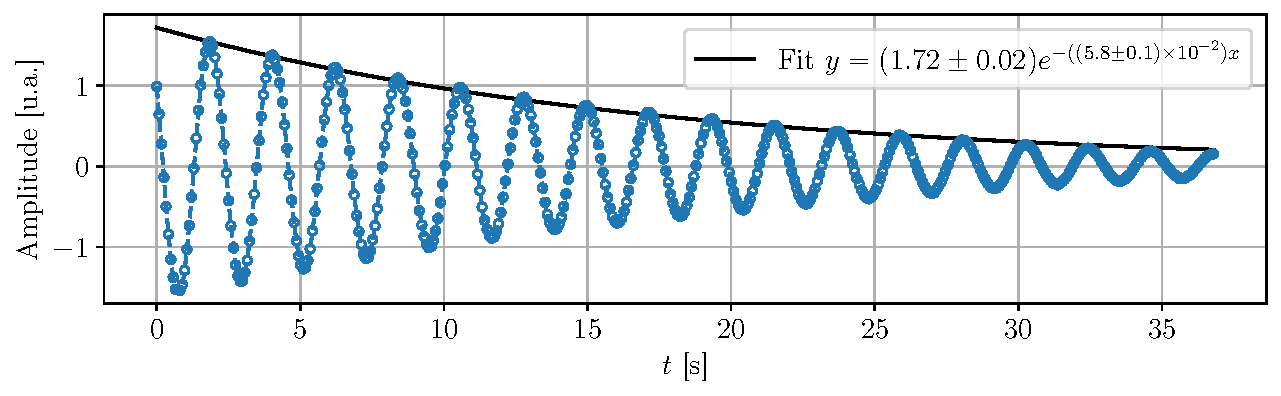
\includegraphics[width=0.98\linewidth]{figures/I3_50_nomot_fitted.pdf}
    \caption{Oscillation libre du disque avec 3 masses supplémentaires et un amortissement de 50\%}
    \label{fig:signal_libre}
\end{figure}

\begin{figure}[h]
    \centering
    \begin{subfigure}{0.48\linewidth}
        \centering
        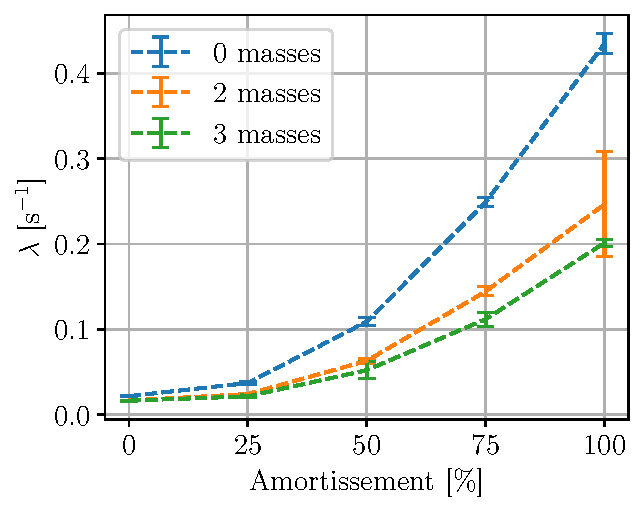
\includegraphics[width=\linewidth]{figures/lambda_nomot.pdf}
        \caption{}
        \label{fig:lambda_libre}
    \end{subfigure}
    \begin{subfigure}{0.48\linewidth}
        \centering
        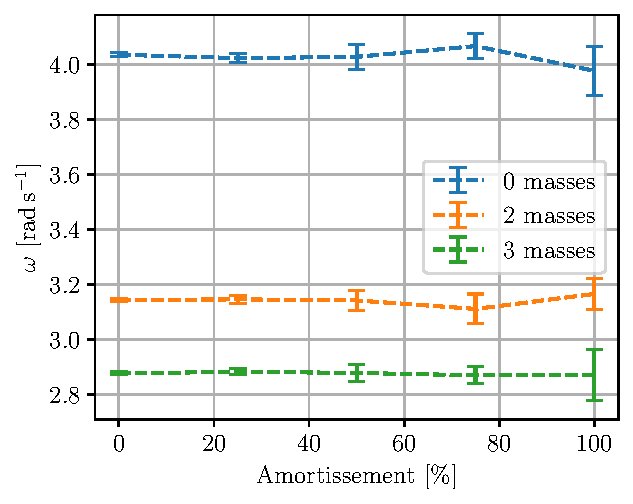
\includegraphics[width=\linewidth]{figures/omega_nomot.pdf}
        \caption{}
        \label{fig:omega_libre}
    \end{subfigure}
    \caption{(a) Le coefficient d'amortissement \(\lambda\) et (b) la pulsation \(\omega\) pour différentes configurations de masses supplémentaires, en fonction de l'amortissement appliqué}
\end{figure}

La pulsation \(\omega_0\) de l'oscillateur harmonique libre sans frottements peut alors être détérminé à partir de l'\autoref{eq:omega_0}. Puisque \(\omega_0\) est censé être constant pour les différents amortissements appliqués, la valeur moyenne a été retenue. Les résultats sont présentés dans le \autoref{tab:omega0_libre}.

\begin{table}[h]
    \centering
    \begin{tabulary}{0.9\linewidth}{C C C C}
        \toprule
        & 0 masses & 2 masses & 3 masses \\
        \midrule
        \(\omega_0\) [\si{\radian\per\second}] & \(4.03 \pm 0.02\) & \(3.14 \pm 0.02\) & \(2.87 \pm 0.02\) \\
        \bottomrule
    \end{tabulary}
    \caption{Valeurs moyennes de la pulsation de l'oscillateur harmonique sans frottements}
    \label{tab:omega0_libre}
\end{table}

\paragraph{Battements transitoires}
Pour les battements dans la solution transitoire de l'\autoref{eq:oscillations_forcees} plusieurs essais de conditions initiales ont été essayés pour le disque à 0 masses et amortissement de 50\%. Le résultat permettant de mieux visualiser les battements est présenté en \autoref{fig:bat_ampl}. Les amplitudes affichées ont été obtenues en prélevant les valeurs absolues des pics minimums et maximums des oscillations. En prenant l'écart entre les deux minimums d'amplitude à $t_1$ et $t_2$ il est possible d'obtenir une période de battement donnant la pulsation de battement expérimentale: $\omega_{B,exp} = (0.426 \pm 0.001)
$ \si{\radian\per\second}.
\begin{figure}[h]
    \centering
    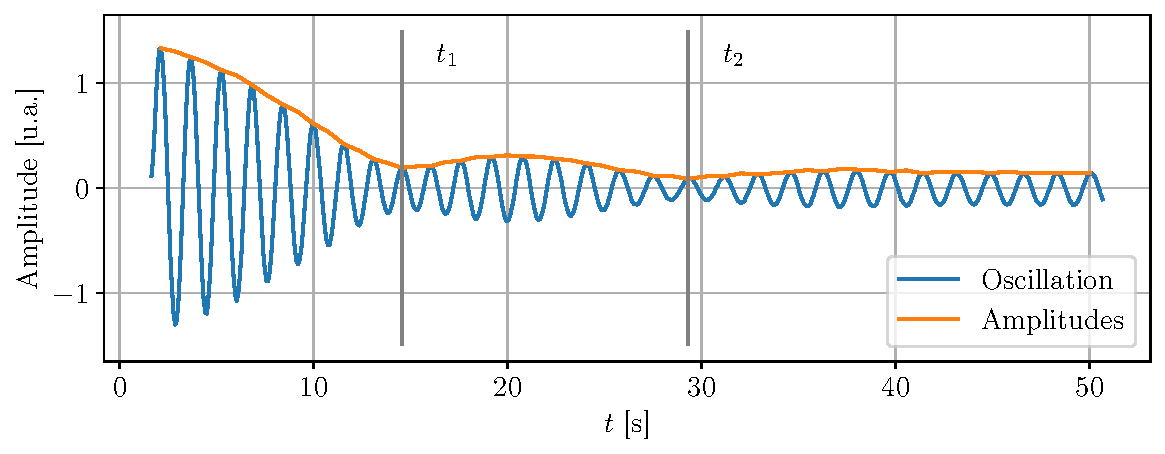
\includegraphics[width=0.9\linewidth]{figures/bat_ampl.pdf}
    \caption{Oscillation forcées du disque et amplitudes avec condition initiale $\theta \gg 1$, 0 masses et un amortissement de 50\%, intervalle d'un battement}
    \label{fig:bat_ampl}
\end{figure}

La transformation de Fourier des signaux du disque et du moteur ont ensuite été prises afin d'obtenir leurs pulsations respectives. Les fonctions obtenues sont présentées en \autoref{fig:bat_fourier}. Deux pics symétriques sont obtenus correspondant à la fréquence $f$ et à $-f$. Cette valeur de $f$ pour les deux signaux permet d'obtenir les pulsations, pour le moteur \hbox{$\Omega = (3.5\pm0.1)$ \si{\radian\per\second}} et pour les oscillations $\omega = (3.8 \pm 0.1)$ \si{\radian\per\second}. Cela donne en utilisant la formule \hbox{\(\omega_{B,th} = |\omega- \Omega| = (0.4\pm0.2)\) \si{\radian\per\second}}. L'écart relatif entre $\omega_{B,exp}$ et $\omega_{B,th}$ par rapport à $\omega_{B,th}$ est donc de 10\%.
\begin{wrapfigure}{R}{0.5\linewidth}
    % \vspace*{-0.5cm}
    \centering
    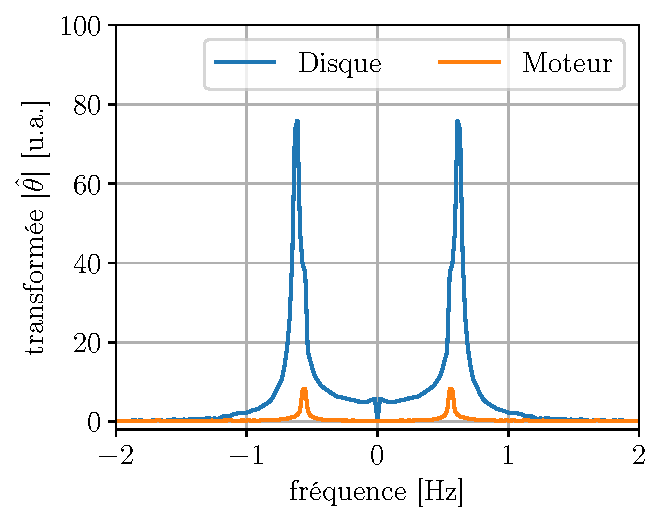
\includegraphics[width=\linewidth]{figures/bat_fourier.pdf}
    \caption{Transformation de Fourier des oscillations du disque et du moteur}
    \label{fig:bat_fourier}
    %%%%% WARNING %%%%%%%
    \vspace*{-0.2cm}
\end{wrapfigure}


\paragraph{Résonance}
Afin de caractériser la résonance, 30 relevés d'oscillations permanentes ont été faits avec le disque sans masse et 75\% d'amortissement. Pour chacun l'amplitude moyenne $A$ a été relevé comme précédemment. La pulsation $\Omega$ et le déphasage $\psi_\mathrm{exp}$ entre le signal du moteur et l'oscillation ont été relevé grâce aux transformées de Fourier des deux signaux, la valeur de $\Omega$ étant la même pour les deux et le déphasage étant l'écart d'angle entre les transformées à la fréquence d'oscillation. Les résultats sont présentés en \autoref{fig:resonance} avec la fonction $\psi_\mathrm{th}$ calculées avec l'\autoref{eq:A_et_psi} et les valeurs de $\lambda$ et $\omega_0$ déterminées grâce aux oscillations libres. Pour $\psi$ la fonction \texttt{angle} de \texttt{numpy} ayant retourné des valeurs entre $-\pi/2$ et $\pi/2$ un décalage de $\pi$ de toutes les valeurs inférieures à 0 a été effectué. Il est possible d'extraire la valeur de la pulsation de résonance $\Omega_r = 4.1\pm0.1$ \si{\radian\per\second} de la \autoref{fig:res_A}.

\begin{figure}[h]
    \centering
    \begin{subfigure}{0.48\linewidth}
        \centering
        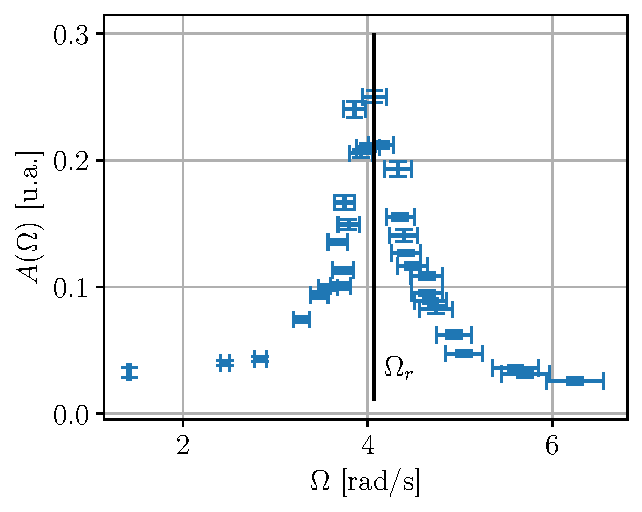
\includegraphics[width=\linewidth]{figures/resonance_A.pdf}
        \caption{}
        \label{fig:res_A}
    \end{subfigure}
    \begin{subfigure}{0.48\linewidth}
        \centering
        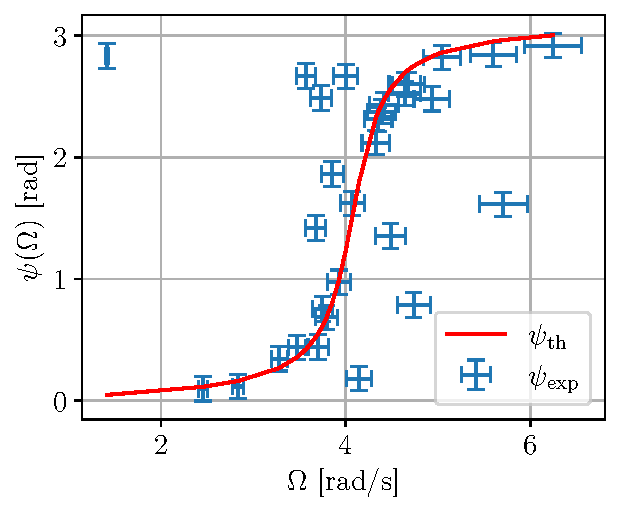
\includegraphics[width=\linewidth]{figures/resonance_psi.pdf}
        \caption{}
        \label{fig:res_psi}
    \end{subfigure}
    \caption{(a) Amplitude des oscillations $A$ et (b) déphasage par rapport au moteur $\psi$, théorique et expérimental, du disque en fonction de la pulsation $\Omega$}
    \label{fig:resonance}
\end{figure}

Les valeurs de $\lambda$ et $\omega_0$ des oscillations libres ont également permis de déterminer $\omega = \sqrt{\omega_0^2 - \lambda^2}$ afin de calculer $\Delta \Omega$ et $Q$. Les valeurs obtenues sont:
\[
    \Delta \Omega = \frac{2 \lambda \omega}{\Omega_r} = (0.50\pm0.01) \, \si{\radian\per\second} , \quad Q = \frac{\Omega_r}{\Delta\Omega} = 8.2\pm0.3
\]

